\begin{theorembox}{Theorem (Order Separation by Supremum)}
\begin{theorem}[Order Separation by Supremum]
\label{thm:order-separation-by-supremum}
Let $A,B\subseteq\mathbb{R}$ be nonempty sets such that
\[
  (\forall a\in A)(\forall b\in B)(a\leq b).
\]
Then $A$ is bounded above, $B$ is bounded below, and the real number
$c:=\sup A$ separates $A$ from $B$; that is,
\[
  (\forall a\in A)(\forall b\in B)(a\leq c\leq b).
\]
In particular,
\[
  \sup A\leq\inf B.
\]
\hyperref[prf:order-separation-by-supremum]{Go to proof.}
\end{theorem}
\end{theorembox}
\begin{remark*}[Standard quantified statement]
\[
\forall A,B\subseteq\mathbb{R}\;
\Bigl[
(A\ne\varnothing\land B\ne\varnothing\land
\forall a\in A\;\forall b\in B\;(a\le b))
\Longrightarrow
\exists c\in\mathbb{R}\;\forall a\in A\;\forall b\in B\;(a\le c\le b)
\Bigr].
\]
\end{remark*}
\begin{remark*}[Predicate reading]
\[
A,B\subseteq\mathbb{R},\qquad P_{\mathbb{R}}=\mathsf{OrderedSet}(\mathbb{R},\leq),
\]
\[
\bigl(A\ne\varnothing\land B\ne\varnothing\land
\forall a\in A\;\forall b\in B\;(a\le b)\bigr)
\Longrightarrow
\operatorname{HasDedekindSeparator}(A,B,P_{\mathbb{R}}).
\]
Equivalently, there exists $c\in\mathbb{R}$ such that
\(\operatorname{IsDedekindSeparator}(c,A,B,P_{\mathbb{R}})\).
\end{remark*}
\begin{remark*}[Negated quantified statement]
\[
\exists A,B\subseteq\mathbb{R}\;
\Bigl[
A\ne\varnothing\land B\ne\varnothing\land
\forall a\in A\;\forall b\in B\;(a\le b)
\land
\forall c\in\mathbb{R}\;\exists a\in A\;\exists b\in B\;(c<a\lor b<c)
\Bigr].
\]
\end{remark*}
\begin{remark*}[Negation predicate reading]
\[
A,B\subseteq\mathbb{R},\qquad P_{\mathbb{R}}=\mathsf{OrderedSet}(\mathbb{R},\leq),
\]
\[
\bigl(A\ne\varnothing\land B\ne\varnothing\land
\forall a\in A\;\forall b\in B\;(a\le b)\bigr)
\land\neg\operatorname{HasDedekindSeparator}(A,B,P_{\mathbb{R}}).
\]
\end{remark*}

\begin{remark*}[Failure modes]
\begin{description}
  \item[Exposition.]
  Failure is witnessed by the displayed negated or contrapositive condition.

  \item[\mathsf{OrderedSet}.]
  \[
\exists A,B\subseteq\mathbb{R}\;
\Bigl[
A\ne\varnothing\land B\ne\varnothing\land
\forall a\in A\;\forall b\in B\;(a\le b)
\land
\forall c\in\mathbb{R}\;\exists a\in A\;\exists b\in B\;(c<a\lor b<c)
\Bigr].
\]
\[
A,B\subseteq\mathbb{R},\qquad P_{\mathbb{R}}=\mathsf{OrderedSet}(\mathbb{R},\leq),
\]
\end{description}
\end{remark*}
\begin{remark*}[Interpretation]
If one nonempty set lies entirely to the left of another, completeness supplies
a real separator between them.
\end{remark*}
\begin{dependencies}
\hyperref[def:reals]{Real Numbers};
\hyperref[def:ordered-set]{Ordered Set};
\hyperref[def:subset]{Subset};
\hyperref[def:real-upper-bound]{Upper Bound};
\hyperref[def:supremum]{Supremum};
\hyperref[ax:completeness-of-reals]{Completeness of $\mathbb{R}$}.
\end{dependencies}
\begin{figure}[htbp]
\centering
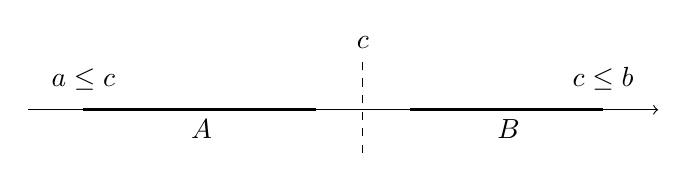
\begin{tikzpicture}[x=1cm,y=1cm]
  \draw[->] (-4,0) -- (4,0);
  \draw[very thick] (-3.3,0) -- (-0.35,0);
  \draw[very thick] (0.85,0) -- (3.3,0);
  \draw[dashed] (0.25,-0.55) -- (0.25,0.65);
  \node[below] at (-1.8,0) {$A$};
  \node[below] at (2.1,0) {$B$};
  \node[above] at (0.25,0.65) {$c$};
  \node[above] at (-3.3,0.12) {$a\le c$};
  \node[above] at (3.3,0.12) {$c\le b$};
\end{tikzpicture}
\caption{A separator $c$ lies between every point of the left set and every point of the right set.}
\end{figure}


\begin{theorembox}{Theorem (Dedekind Cut Property)}
\begin{theorem}[Dedekind Cut Property]
\label{thm:dedekind-cut-property}
Let $L,U\subseteq\mathbb{R}$ be nonempty sets satisfying
\[
  L\cap U=\varnothing,
  \qquad
  L\cup U=\mathbb{R},
\]
and
\[
  (\forall \ell\in L)(\forall u\in U)(\ell<u).
\]
Then either $L$ has a maximum or $U$ has a minimum.  Equivalently,
\[
  \max L\text{ exists}
  \qquad\text{or}\qquad
  \min U\text{ exists}.
\]
\hyperref[prf:dedekind-cut-property]{Go to proof.}
\end{theorem}
\end{theorembox}
\begin{remark*}[Standard quantified statement]
\[
\forall A,B\subseteq\mathbb{R}\;
\Bigl[
(A,B\ne\varnothing\land A\cup B=\mathbb{R}\land A\cap B=\varnothing
\land \forall a\in A\;\forall b\in B\;(a<b))
\Longrightarrow
\exists c\in\mathbb{R}\;\forall a\in A\;\forall b\in B\;(a\le c\le b)
\Bigr].
\]
\end{remark*}
\begin{remark*}[Predicate reading]
\[
A,B\subseteq\mathbb{R},\qquad P_{\mathbb{R}}=\mathsf{OrderedSet}(\mathbb{R},\leq),
\]
\[
\operatorname{IsDedekindSeparation}(A,B,P_{\mathbb{R}})\Longrightarrow
\operatorname{HasDedekindSeparator}(A,B,P_{\mathbb{R}}).
\]
Equivalently, the conclusion supplies some $c\in\mathbb{R}$ with
\(\operatorname{IsDedekindSeparator}(c,A,B,P_{\mathbb{R}})\).
\end{remark*}
\begin{remark*}[Negated quantified statement]
\[
\exists A,B\subseteq\mathbb{R}\;
\bigl(\operatorname{IsDedekindSeparation}(A,B,\mathbb{R})\land
\neg\operatorname{HasDedekindSeparator}(A,B,\mathbb{R})\bigr).
\]
\end{remark*}
\begin{remark*}[Negation predicate reading]
\[
A,B\subseteq\mathbb{R},\qquad P_{\mathbb{R}}=\mathsf{OrderedSet}(\mathbb{R},\leq),\qquad
\operatorname{IsDedekindGap}(A,B,P_{\mathbb{R}}).
\]
\end{remark*}

\begin{remark*}[Failure modes]
\begin{description}
  \item[Exposition.]
  Failure is witnessed by the displayed negated or contrapositive condition.

  \item[\operatorname{IsDedekindSeparation} / \operatorname{HasDedekindSeparator}.]
  \[
\exists A,B\subseteq\mathbb{R}\;
\bigl(\operatorname{IsDedekindSeparation}(A,B,\mathbb{R})\land
\neg\operatorname{HasDedekindSeparator}(A,B,\mathbb{R})\bigr).
\]
\[
A,B\subseteq\mathbb{R},\qquad P_{\mathbb{R}}=\mathsf{OrderedSet}(\mathbb{R},\leq),\qquad
\operatorname{IsDedekindGap}(A,B,P_{\mathbb{R}}).
\]
\end{description}
\end{remark*}
\begin{remark*}[Interpretation]
The real line has no ordered partition into a left part and a right part with
an unfilled gap between them.
\end{remark*}
\begin{dependencies}
\hyperref[def:reals]{Real Numbers};
\hyperref[def:ordered-set]{Ordered Set};
\hyperref[def:subset]{Subset};
\hyperref[def:union]{Union};
\hyperref[def:intersection]{Intersection};
\hyperref[thm:order-separation-by-supremum]{Order Separation by Supremum}.
\end{dependencies}

\begin{corollarybox}{Corollary (No Gaps in $\mathbb{R}$)}
\begin{corollary}[No Gaps in $\mathbb{R}$]
\label{cor:no-gaps-in-r}
Let $L,U\subseteq\mathbb{R}$ be nonempty sets satisfying
\[
  L\cap U=\varnothing,
  \qquad
  L\cup U=\mathbb{R},
\]
and
\[
  (\forall \ell\in L)(\forall u\in U)(\ell<u).
\]
Then there exists a unique $c\in\mathbb{R}$ such that exactly one of the
following alternatives holds:
\[
  L=\{x\in\mathbb{R}:x<c\},
  \qquad
  U=\{x\in\mathbb{R}:c\leq x\},
\]
or
\[
  L=\{x\in\mathbb{R}:x\leq c\},
  \qquad
  U=\{x\in\mathbb{R}:c<x\}.
\]
Thus every Dedekind cut of $\mathbb{R}$ is determined by a real number.
\hyperref[prf:no-gaps-in-r]{Go to proof.}
\end{corollary}
\end{corollarybox}
\begin{remark*}[Standard quantified statement]
\[
\neg\exists A,B\subseteq\mathbb{R}\;\operatorname{IsDedekindGap}(A,B,\mathbb{R}).
\]
\end{remark*}
\begin{remark*}[Predicate reading]
\[
P_{\mathbb{R}}=\mathsf{OrderedSet}(\mathbb{R},\leq),\qquad
\operatorname{IsOrderComplete}(P_{\mathbb{R}}).
\]
\end{remark*}
\begin{remark*}[Negated quantified statement]
\[
\exists A,B\subseteq\mathbb{R}\;\operatorname{IsDedekindGap}(A,B,\mathbb{R}).
\]
\end{remark*}
\begin{remark*}[Negation predicate reading]
\[
P_{\mathbb{R}}=\mathsf{OrderedSet}(\mathbb{R},\leq),\qquad
\neg\operatorname{IsOrderComplete}(P_{\mathbb{R}}).
\]
\end{remark*}

\begin{remark*}[Failure modes]
\begin{description}
  \item[Exposition.]
  Failure is witnessed by the displayed negated or contrapositive condition.

  \item[\operatorname{IsDedekindGap} / \operatorname{IsOrderComplete}.]
  \[
\exists A,B\subseteq\mathbb{R}\;\operatorname{IsDedekindGap}(A,B,\mathbb{R}).
\]
\[
P_{\mathbb{R}}=\mathsf{OrderedSet}(\mathbb{R},\leq),\qquad
\neg\operatorname{IsOrderComplete}(P_{\mathbb{R}}).
\]
\end{description}
\end{remark*}
\begin{remark*}[Interpretation]
Every Dedekind separation of the real line is accounted for by a real boundary
point.
\end{remark*}
\begin{dependencies}
\hyperref[def:reals]{Real Numbers};
\hyperref[def:ordered-set]{Ordered Set};
\hyperref[thm:dedekind-cut-property]{Dedekind Cut Property}.
\end{dependencies}
